\documentclass[conference]{IEEEtran}
\IEEEoverridecommandlockouts
% The preceding line is only needed to identify funding in the first footnote. If that is unneeded, please comment it out.
\usepackage{cite}
\usepackage{amsmath,amssymb,amsfonts}
\usepackage{algorithmic}
\usepackage{graphicx}
\usepackage{textcomp}
\usepackage{xcolor}
\usepackage{lipsum}
\usepackage[utf8]{inputenc}
\usepackage[english]{babel}
\def\BibTeX{{\rm B\kern-.05em{\sc i\kern-.025em b}\kern-.08em
    T\kern-.1667em\lower.7ex\hbox{E}\kern-.125emX}}
\begin{document}

\title{Parkinson's disease prediction using vocal parameters\\
}

\author{\IEEEauthorblockN{Manideep karne}
\IEEEauthorblockA{\textit{700725935} \\
\textit{dept.Computer Science}\\
\textit{University of Central Missouri} \\
karnemanideep@gmail.com}
\and
\IEEEauthorblockN{Nikhil Manikya}
\IEEEauthorblockA{\textit{700734200} \\
\textit{dept.Computer Science}\\
\textit{University of Central Missouri} \\
 nmanikya853@gmail.com}
 \\ 
\linebreakand
\IEEEauthorblockN{Ashlesh Marneni}
\IEEEauthorblockA{\textit{700742493} \\
\textit{dept.Computer Science}\\
\textit{University of Central Missouri} \\
ashleshraomarneni@gmail.com}
\and
\IEEEauthorblockN{Vamsi Sairam Adi}
\IEEEauthorblockA{\textit{700741207} \\
\textit{dept.Computer Science}\\
\textit{University of Central Missouri} \\
adivamsi2000@gmail.com}
}

\maketitle
\begin{abstract}
Parkinson’s disease is the second most  dangerous neurodegenerative disease that affects the elderly people after Alzheimer's disease. Around 1 million people are diagnosed with Parkinson's disease in the USA now. Since this is a neuro degenerative disease early detection of the disease helps in timely treatment and in turn it improves the life expectancy of the patients.The progression of disease develops several symptoms in the patient one of the noticeable symptoms are voice changes.  There are several methods to diagnose the disease; one of the novel approaches is predicting the disease from vocal parameters. This disease affects the jaw movements which results in changes of pitch and intensity of the voice.Vocal impairment is one of the early signs of Parkinson’s disease. From the collected voice we breakdown the vocal features.With the help of machine learning methods we find the patterns in the data.Since the dataset has a combination of features frequency , intensity, HNR and NHR.  Few parameters are measured in frequency and few are measured in ratios. The challenging task is to predict the best features from the data.
We apply non linear dimensionality reduction method i.e. PCA to extract the features
After the reduction of features we apply tree based algorithms to classify the disease PD or healthy.

\end{abstract}
\footnote{\href {https://github.com/Manideepkarne/Machine-Learning-Final-project-.git}}
\begin{IEEEkeywords} HNR(Harmonic to Noise Ratio),neuro degenerative, NHR(Noise to Harmonic Ration),Non linear dimentionality reduction,PCA(Principal Component Analysis) and tree based algorithms,
\end{IEEEkeywords}

\section{Introduction}
Parkinson’s disease is a neuro system disorder that affects functions like speech, writing and moments of muscles. Major challenges for diagnosing the disease are: It is very difficult to  find the symptoms in early stages and the symptoms of this disease overlap with the other neuro diseases.This disease affects the person’s motor and non motor skills. If this disease is identified in the early stages the mortality rate of the patient can be increased significantly. In the list of symptoms one of the main differentiable symptoms are speech impairment since the disease affects the functioning of jaw muscles this condition leads to changes in voice and pitch of the patient.Though this is an identifiable symptom it is challenging task to identify with voice sample with the invention of machine learning as the core functioning is find n the patterns in the data.Parkinson’s disease is the second most  dangerous neurodegenerative disease that affects the elderly people after Alzheimer's disease. Around 1 million people are diagnosed with Parkinson's disease in the USA now. Since this is a neuro degenerative disease early detection of the disease helps in timely treatment and in turn it improves the life expectancy of the patient

Parkinson’s disease is a neurodegenerative disorder which develops the symptoms slowly. In this study researchers explored various machine learning classifiers to predict Parkinson's disease. With the acoustic parameters of the subject passed to the model which is created using multiple classifiers Logistic regression, KNN classifier,Naive Bayes classifier  and Random Forest classifier. Among the 3 classifiers KNN performed better with 94 percent accuracy .
Parkinson's disease can be identified through vocal or acoustic parameters of the PD patient.This can be identified from the stressing of vowels and consonant sounds.For this experiment MLP(Multi Layer Perceptron) and Logistic regression models are implemented to check the performance and the results show that AUC-ROC is 82 percent.
Main features in the voice parameters are jitter, shimmer, DFA,PPE(pitch period entropy) are some of the important features in a voice measure.On this data various machine learning models are implemented Bagging and Boosting models.According to the results analysis Light BGM achieved highest accuracy of 95 percent .
A comparative study is conducted to check the performance of the machine learning models.In the comparative study the speed of the models is analyzed , accuracy of the predictions and assessed  the suitability of the problem.After analysis this is deployed as an application.Research suggests that 90 percent of the PD patients experience speech impairment and voice disorders. Some of the symptoms are breathiness in the voice, monotone of the voice, in appropriate articulation, soft voice that is low intensity and hoarse voice. Because of these symptoms patients won’t participate in social interactions due to lack of confidence.


In this paper we are proposing a machine learning model to predict the class of Parkinson’s disease using smartphone voice samples data.The data contains various components of the subject voice frequency, pitch,intensity in various measures.Each voice record of the subject is broken into 512 components which is high dimensional data. These records contain both healthy and patient records.The project is divided into 2 steps one is dimensionality reduction method and the other one is classification.The dimensionality reduction is achieved through PCA method and classification is implemented using machine learning ensemble models XGBoost and Gradient Boosting algorithms. The performance of the models is evaluated based on several metrics including accuray.

PCA is a dimensionality reduction method which reduces the dimensions of the data and preserves most of the information. In most of the cases reducing dimensions comes at the cost of losing the information. In most of the cases important information also.In case of PCA we preserve the data as much as possible and reduce dimensions also.
The steps of PCA as follows:
1.Standardizing the data:
We need to standardize the data since the data in further steps of PCA will become more vulnerable, which data with highest ranges will dominate the lower range data so we will normalize the data.
2.Covariance matrix:
In this step we calculate the covariance matrix. This is to measure the variance of the data points from the mean with respect to each other.In this step if the variables are highly correlated those are considered as redundant variables and those can be ignored.
3.Computing Eigenvalues and Eigenvectors:
From the covariance matrix we calculate eigen values and eigen vectors with the help of these we calculate the principal components.
4.Principal components:
Principal components are the new vectors which are formed from the linear combination of the existing values with largest possible variance.
5.Forming a feature vector:
In this step we form a feature vector with the help of eigen values and eigen vectors.First we sort the eigenvalues in the descending order and we decide whether we have to discard the less significant values or retain them in order to calculate the principal components.

XGBoost algorithm is an Extreme Gradient Boosting algorithm which is an ensemble model which uses the predictions of the weak learners and combines those predictions to produce quality predictions. XGBoost is used in many real world applications as it handles large amounts of data very well and it has preprocessing in built.functionality.
Gradient Boost:
Gradient boosting is also an ensemble model which has the sequential models for predictions.In this case the predictions of the later model is improved compared to the previous model.
The advantages of this algorithm are speedy predictions with high accuracy.

Gradient boosting algorithm and AdaBoost algorithms are the boosting ensemble methods. In gradient boosting method the algorithms is fixed that decision tree where as in AdaBoost we can explicitly mention the algorithms names but the number of estimator in the AdaBoost is 100 by default. Gradient Boosting algorithm is used for both kind of problems regression and classification.
Another type of ensemble algorithms are voting classifiers in this we use statistical methods to predict. In the voting classifiers again we have  two different classification types one is hard voting and the other one soft voting.
Bagging methods are also known as bootstrap aggregation. In the bagging method total samples are divided into sub samples and the predictions are selected based on the aggregation. The main objective of the bagging method is to reduce the variance of the algorithms. For example decision tree like algorithms are sensitive to the never seen samples because these are trained on the sub samples. So to avoid that problem we take the aggregation of the data.
Support Vector Machine is a supervised machine learning algorithm which acts as a regressor and classifier.In our problem we have a classification task which separates the two classes by a hyperplane. This is implemented using the scikit-learn library. There are hyper parameters to tune the SVM algorithm.
C: regularisation parameter
Kernel : different types of kernel used in the algorithm's default kernel is ‘rbf’ and the other types of the kernels are linear, ploy, sigmoid and precomputed.
degree:Degree of the polynomial kernel default value is 3 and non negative value.
Maxiter: Maximum number of iterations default value is -1
Probability :if the predictions wants to be in the probability then the value needs to be specified as True.
Gamma: gamma values are scale and auto.

The performance of the models is evaluated using following parameters:
Accuracy,Precision, Recall, F1 score, AUC-ROC curve and Confusion matrix

Gradient boosting and RandomForest:
The first step in Gradient Boosting is to build the base or weak learner. Second step is to calculate the residuals which is  calculated by subtracting the observed value from the predicted value.If the residual value is positive we follow along and move to the next phase and if the value is negative then the flow goes backwards, learns and then moves forward.
RandomForest is also a boosting method which is a collection of decision trees.
RandomForest pseudocode:
\begin{itemize}
    \item 1.Randomly select “k” features from total “m” features.(Where k << m)
    \item 2.Among the “k” features, calculate the node “d” using the best split point.
    \item 3.Split the node into daughter nodes using the best split.
    \item 4.Repeat 1 to 3 steps until “l” number of nodes has been reached.
    \item 5.Build forest by repeating steps 1 to 4 for “n” number times to create “n” number of trees.
    \item 6.Takes the test features and use the rules of each randomly created decision tree to predict the outcome and stores the predicted outcome (target)
    \item 7.Calculate the votes for each predicted target.
    \item 8.Consider the highly voted predicted
\end{itemize}





 target as the final prediction from the random forest algorithm.
RandomForest has various applications in banking, medicine, stock market, e-commerce.




\section{Motivation}
Research suggests that 90 percent of the PD patients experience speech impairment and voice disorders. Some of the symptoms are breathiness in the voice, monotone of the voice, in appropriate articulation, soft voice that is low intensity and hoarse voice. Because of these symptoms patients won’t participate in social interactions due to lack of confidence. With decreased communication affects the patient's quality of life since communication is the key in everyone’s life. Once the patient or relatives notice the changes in voice of the patient they can book the appointment with a speech therapist but the availability of the therapist in some locations is scarce and rare to find. A virtual and automated speech impairment recogniser will be a great help to the PD patients.
So  we are implementing automated machine learning models to detect the voice changes of the PD patient and normal people using some useful voice parameters.



\\

\section{Objectives}
Though PCA is used for dimensionality reduction in both supervised and unsupervised learning. PCA works well in unsupervised learning. In case of supervised learning, it leads to data leakage and sometimes it will not create the new axis with discriminant features. To tackle this problem we use tree based algorithms which increases the variability and reduces the data leakage.

\begin{itemize}
    \item Analysing the data and cleaning the data
    \item In ourproject we have used  various voice parameters of the data which vary in measurement and units.
    \item standardizing the data and applying PCA to reduce the dimentions of the data
    \item The objective of our project is to predict Parkinson's disease using decision tree and XGBoost  classifiers comparing the results 
    \item concluding the project and mentioning the future work
    \item Selecting the best algorithms considering them for future work
\end{itemize}

\section {Related work}

Parkinson’s disease is a neuro degenerative disease which occurs due to reduced production of dopamine in the brain. One of the motor symptoms that appear in the PD patient are tremors and shivers. One of the solutions to these tremors is using DBS(Deep Brain Stimulation) and the drawback is that though we apply these stimulation methods in the beginning they work fine and control the tremors in the patients but after a period of time the symptoms reappear.  So in our paper we are proposing a method to find the stage of Parkinson's disease and when the DBS(Deep Brain stimulation) needs to be started. This whole process is executed using mathematical tools and the Markov process using the medical parameters\cite{7391433}.

Nearly 6.3million people are diagnosed with Parkinson's disease across the world. Researchers suggest that 90  percent of the patients are suffering from motor skills impairment. In this study we are experimenting with a machine learning method to classify the PD and healthy individuals. To extract the features of wave like clock drawing test Histogram Oriented Gradients(HOG) features. This disease doesn’t have a cure but the early detection of the disease can reduce the progression of the disease and the patient can opt for the relevant therapies. In this paper we are proposing Artificial Neural Networks and Random Forest classifiers to classify the data\cite{10047447}.

Parkinson’s disease is caused due to the damaged neurons which decreases the production of dopamine in the brain. Reduced production of dopamine, people can not control simple activities. In this paper we are implementing the Radial basis function to predict the progression of the disease. On the data of Total unified parkinson’s disease data the model achieved 97 percent accuracy\cite{9971828}.

Finding the symptoms of Parkinson’s disease in the early stage is a challenging task. This is a challenging task to even the doctors. After reaching a certain stage we can predict the symptoms of the disease. So an automated tool to predict the disease acts as a great help to the doctors and the patients. In this study we are proposing multiple machine learning models to predict the presence of the disease. The experiment is conducted on the UCI machine learning repository parkinson’s voice data \cite{9298033}.

Nowadays a large number of countries are experiencing neuro patients across the world. In this paper we are proposing a model i.e. multimodal neuro disorder prediction.In this study the main objectives of the project are:1. Detection and prediction of Alzheimer’s disease 2. Prediction of Parkinson’s disease 3. Generalised anxiety detection and stress detection\cite{10007434}.

These days computer aided diagnosis or Medical Signal Processing are gaining popularity. In this study we are proposing a machine learning model to predict the presence of the disease using Convolutional Neural Networks(CNN) and ANN(Artificial Neural Networks) and calculate the evaluation parameters like sensitivity, specificity and accuracy of the models. CNN model scored highest accuracy of 93.7 percent\cite{9493456}.

Elderly people are the main age group that are affected by Parkinson’s disease, especially people above 60 years of age. In the existing system the prediction system of the disease mainly depends on the clinical parameters of the patient. Analysing large amounts of the clinical data depends on the clinicians which is also a cumbersome task. To avoid the above problems we are proposing an auxiliary clinical evaluation of the disease using machine learning methods. To implement  machine learning methods we have deployed Naive Bayes, KNN and Random Forest algorithms. In the traditional methods a single weak learner model is implemented to predict the results. In this study we are implementing the ensemble model to predict the disease using the above algorithms. This novel approach proved that there is an improved accuracy when compared to the single model predictions\cite{9763618}.	

The exact cause of Parkinson's disease is still not known. But recent studies strongly believe that analysing genetic and environmental factors of the people gives a better understanding of the data and in some cases these are the direct factors that affect the disease cause. The main challenge in analysing the gensim data is it is highly distorted and clumsy.  In this study we have collected both the categories of the data and preprocessed and cleaned the data using R tools which improved the accuracy of the models. In this study we have followed the computational approach\cite{9315926}.

Parkinson’s disease is a neuro degenerative disease which spreads exponentially with the increase in severity. Patients with PD can not perform simple tasks even walking, eating and communicating properly. The important task here is finding the severity stage of the disease.  In this study we are proposing a model which predicts the severity of the disease and its progression. To predict this we are implementing a hybrid neural network structure i.e. CNN with Random Forest classifier\cite{9456292}.

Predicting the disease from voice parameters is a challenging task. The patient voice parameters are broken down into useful parameters. They come in high dimensions that is 754 in the current scenario. If  we use the raw data to train the model the complexity of the model is increased drastically. There are multiple methods to reduce the dimensions of the data. One is feature selection. In this method the model selects best features based on the variance during this process there is a chance of losing the information. To overcome this problem we have introduced a nonlinear dimensionality reduction method that is PCA which uses the existing features linear combination to produce the new features. After reducing the dimensions we have applied an Artificial Neural Network classifier  to the data\cite{9065876}.

Many studies analysed the genes data but the study focused on either protein gene data or ignore long non-coding genes data. But in this novel approach we are combining both sets of the data to rule out the association of parkinson's data. This proposed system is divided into 4 stages. In the first stage we preprocess the data of DNA FASTA. In the second stage through feature extraction we separate the discriminative features of the data.These extracted features would be fused for the future use. In the third stage, the AdaBoost classifier is used to select the features from the data and also reduces the dimensions of the data. In the Gradient Boosting classifier is used to predict the disease. The model achieved the 87 percent on the test data\cite{10032519}.

Medical datasets come in different dimensions, usually the dimension would be large. In this paper we are proposing a feature selection method to select the features which have high scores. To select the features we are implementing the RFE(Recursive Feature Elimination)method to eliminate the features in the cyclic process and to select the  best features from the data. And the accuracy of the model is achieved through 91 percent accuracy\cite{9791490}.

In this paper we are proposing a model to find the trends in the sleep behaviour in the PD patients and healthy patients. The sleep patterns are recorded using REM sleep behaviour disorder metre and the recordings are classified using Logit model of machine learning\cite{9230918}\cite{6944530}.

Parkinson's disease is very difficult to diagnose due to its varied symptoms and the symptoms of the disease overlap with the other disease symptoms.In this paper we are proposing a system to classify the disease using SVM(Support Vector Machine) classifier to classify the disease using fMRI(Functional Magnetic Resonance Imaging) method.To evaluate the model we are using sensitivity, specificity and F1 score of the model. Our proposed model achieved 99.53 percent accuracy on the test dataset and 100 percent specificity and 99.76 sensitivity which are good results\cite{8365279}\cite{8961441}.

Parkinson’s disease is a progressive disease which slowly develops the symptoms and neuro degenerative disorders need to be treated  in the early stages. The data is divided into two groups one is PD and the other one is healthy group. We have used RFE(Recursive Feature Elimination) to select the best features from the data. In addition to the RFE we have implemented linear and non linear dimensionality reduction methods\cite{9864672}\cite{5545301}.
Though the datasets come in different dimensions the size of the datasets are very small to effectively train the data on the machine learning algorithms. We have used a cross validation technique coupled with RFE(Recursive Feature Elimination) method. We have used 10 crossfolds on the training and testing data.Various machine learning models are implemented Logistic Regression(LR), SVM(Support Vector Machine), ANN(Artificial Neural Networks) , RandomForest(RF) and DT(Decision Tree) are used to classify the data\cite{9832191}\cite{7749257}.

\section{Data Description}\label{AA}
The dataset is collected from open source repository kaggle. The dataset is in the format of ASCII or CSV. The dataset contains the vocal parameters of the patient.Each column represents the one vocal parameter of the patient. There are 195 records.

Attributes description:
\begin{itemize}
    \item name - volunteer name 
    \item MDVP:Fo(Hz) - Average vocal fundamental frequency
    \item MDVP:Fhi(Hz) - Maximum vocal fundamental frequency
    \item MDVP:Flo(Hz) - Minimum vocal fundamental frequency
    \item MDVP:Jitter(perencentage), MDVP:Jitter(Abs), MDVP:RAP, MDVP:PPQ, Jitter:DDP - Several measures of variation in fundamental frequency
    \item MDVP:Shimmer,MDVP:Shimmer(dB),Shimmer:APQ3
    \item Shimmer:APQ5,MDVP:APQ,Shimmer:DDA - measure of variation in amplitude
    \item NHR, HNR - Two measures of the ratio of noise to tonal components in the voice
    \item status - The health status of the subject (one) - Parkinson's, (zero) - healthy
    \item RPDE, D2 - Two nonlinear dynamical complexity measures
    \item DFA - Signal fractal scaling exponent
    \item spread1,spread2,PPE - Three nonlinear measures of fundamental frequency variation
\end{itemize}

\newpage
\section{Proposed Framework}
 \begin{figure}[!h]
     \centering
     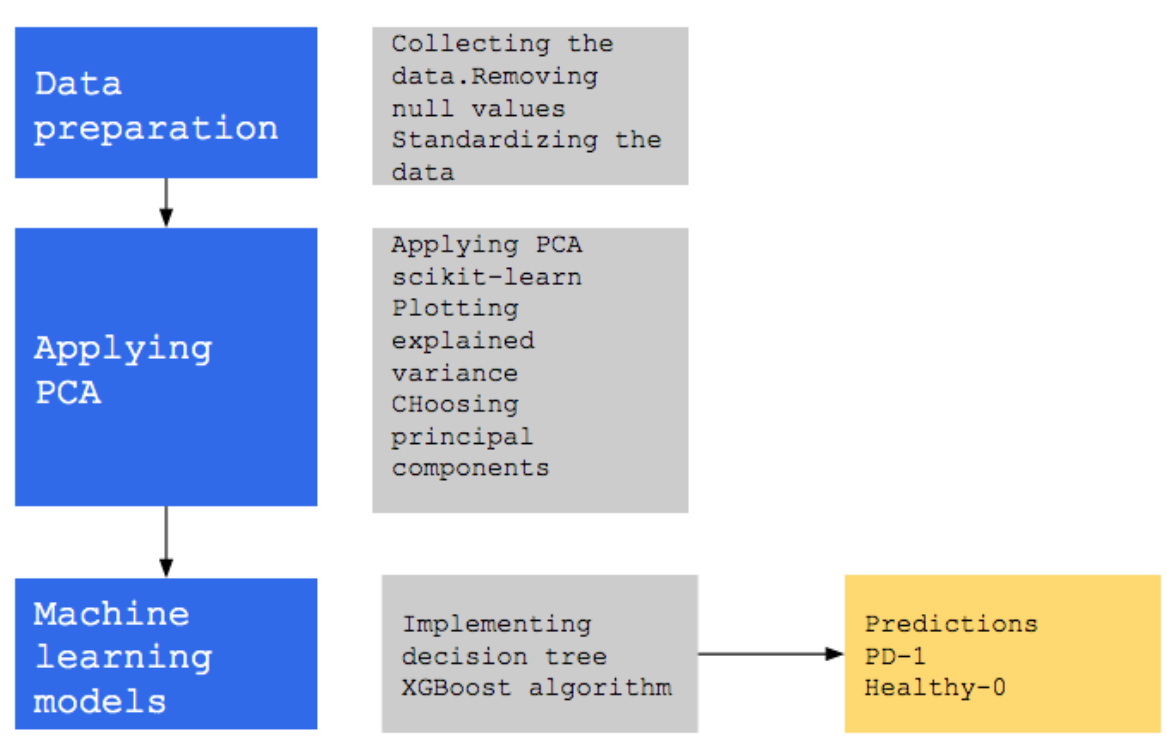
\includegraphics[height=6cm,width=9cm]{WORKFLOW.png}
    \caption{Workflow}
    \label{fig:8}
 \end{figure}
Project is divided into 4 stages i.e. Data preprocessing or data cleaning, Exploratory data analysis, Ensemble modeling and Web deployment.In the first stage raw data is cleaned by removing unnecessary columns, renaming the columns and label encoding the target variables. In the second stage the structure of the data and observations are drawn from the visualizations.In the third stage cleaned data is forwarded to the ensemble models.Best performing model is chosen amongst the 3 models.For a given data predictions are shown using Python web interface.

Preprocessed data is split into train and test in the ratio of 80-20 using scikit-learn train test split method. Ensemble' in statistical terms considered as a group of similar systems or group of same systems with different states.The implementation of the project is divided into following steps:
\begin{itemize}
    \item Collecting the dataset 
    \item Cleaning the data 
    \item Exploring the data
    \item Data preparation i.e. standardizing the data and encoding the categorical values
    \item Applying PCA on the standardized data
Plotting the explained variance graph selecting principal components
\item Fitting the data to PCA object with selected components. Implementing the machine learning models
Evaluating the performance of the models
\end{itemize}





\subsection{PCA}
Principal Component Analysis transforms the features from higher dimensional space into lower dimensional space by creating new axes from the existing features. It divides the variance of the features into components, usually the first component contains the maximum amount of variance. Before we transform the data using PCA we need to standardize the data.

  \begin{figure}[!h]
     \centering
     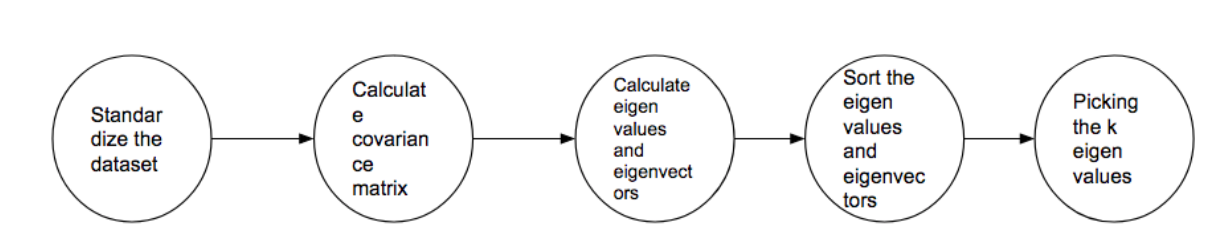
\includegraphics[height=4cm,width=9cm]{pca.png}
    \caption{PCA flow}
    \label{fig:8}
 \end{figure}



\subsection{Tree based algorithms}
In this project we have implemented the Decision tree and XGBoost algorithms to classify the disease. Both the algorithms are implemented using scikit-learn library. Decision tree classifier scored 59 percent accuracy on the test dataset whereas XGBoost scored 62 percent accuracy on the test dataset.


  \begin{figure}[!h]
     \centering
     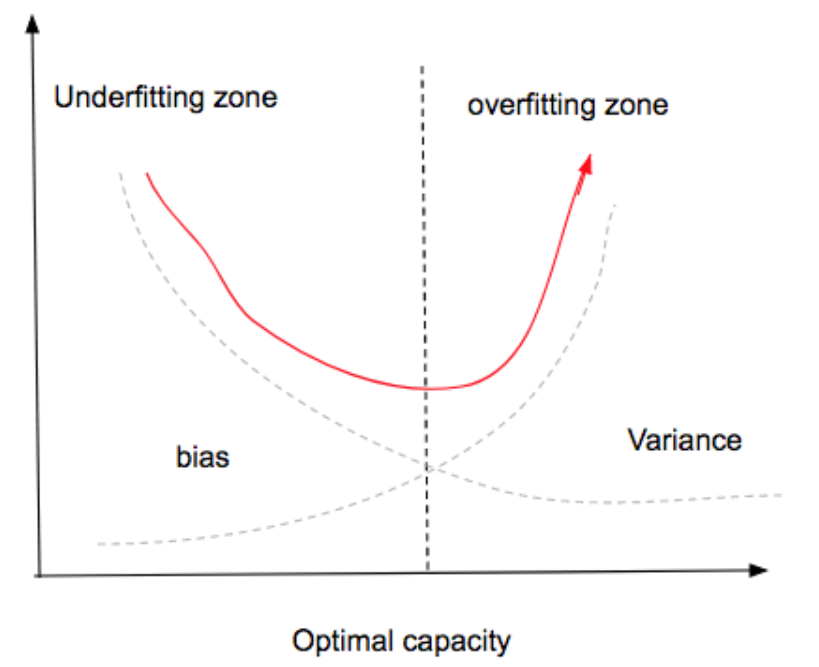
\includegraphics[height=6cm,width=8cm]{bias.png}
    \caption{Bias variance plot for tree algorithms}
    \label{fig:8}
 \end{figure}


 \subsection{Exploratory Data Analysis}
In the exploratory data analysis we have analysed the data and its underlying structure. Following figures show the distribution of the data and outliers presence and histogram distribution of the continous data. Exploratiry data analsis is an important step in machine learning. This helps in which algorithm to apply by understanding the data. There are various plots toexplore the data. Exploratory data analysis is a cyclic process in which user will have some assumptions and check the assumptions whether they are true or not. It can be otherwise also from the visualizations we can draw the conclusions in this case the visualizations are rough or not specific.In our project we have tried two methods first we started with the 


 \begin{figure}[!ht]
     \centering
     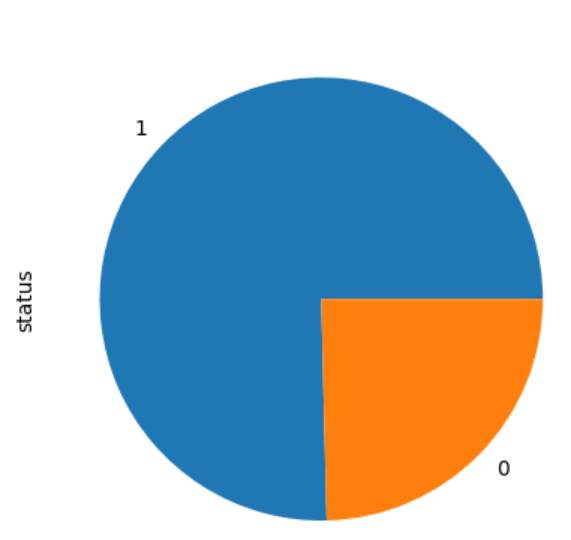
\includegraphics[height=6cm,width=8cm]{distribution.png}
    \caption{target variables distribution}
    \label{fig:8}
 \end{figure}
 
 
 \begin{figure}[!ht]
     \centering
     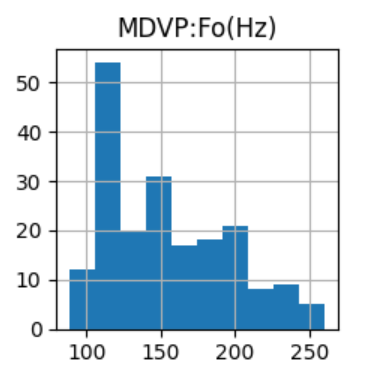
\includegraphics[height=6cm,width=8cm]{mdvp.png}
    \caption{mdvp distribution}
    \label{fig:8}
 \end{figure}

  \begin{figure}[!ht]
     \centering
     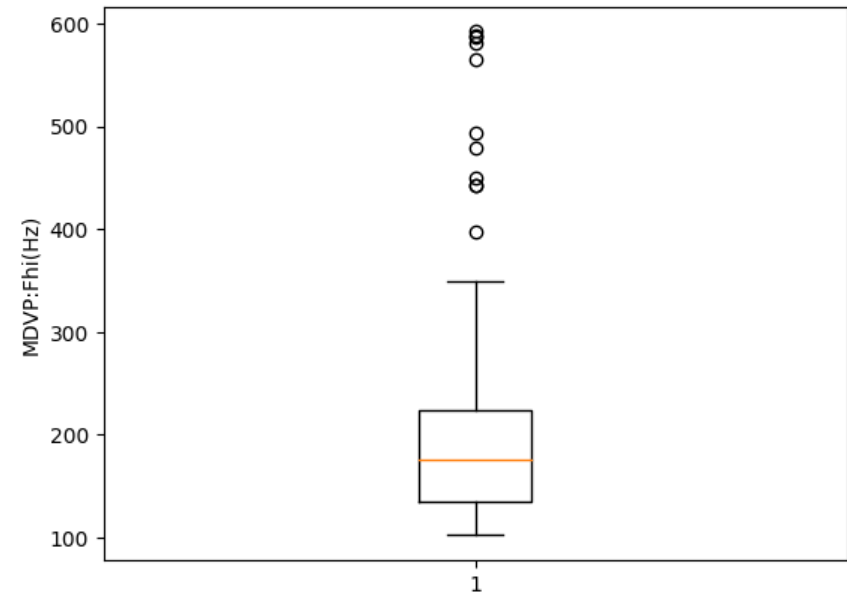
\includegraphics[height=6cm,width=8cm]{mdvp_outliers.png}
    \caption{mdvp boxplot}
    \label{fig:8}
 \end{figure}

 
   \begin{figure}[!ht]
     \centering
     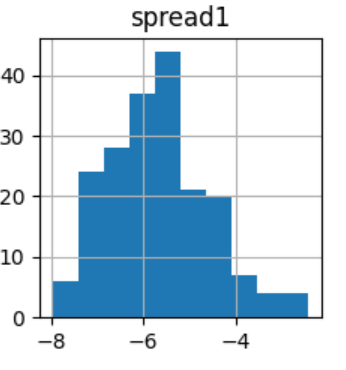
\includegraphics[height=6cm,width=8cm]{spread1.png}
    \caption{spread 1 distribution}
    \label{fig:8}
 \end{figure}


 
   \begin{figure}[!ht]
     \centering
     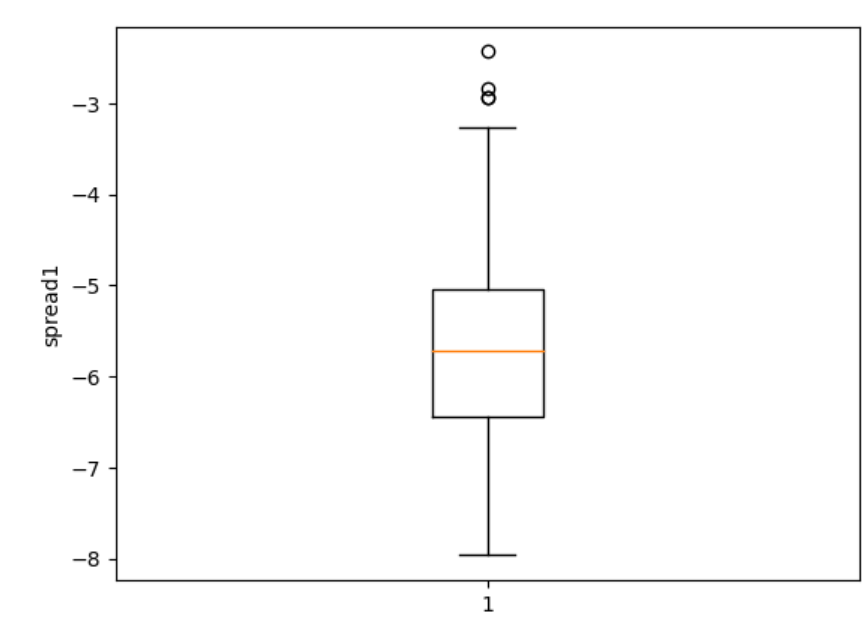
\includegraphics[height=6cm,width=8cm]{spread1_out.png}
    \caption{spread 1 boxplot}
    \label{fig:8}
 \end{figure}

  
   \begin{figure}[!ht]
     \centering
     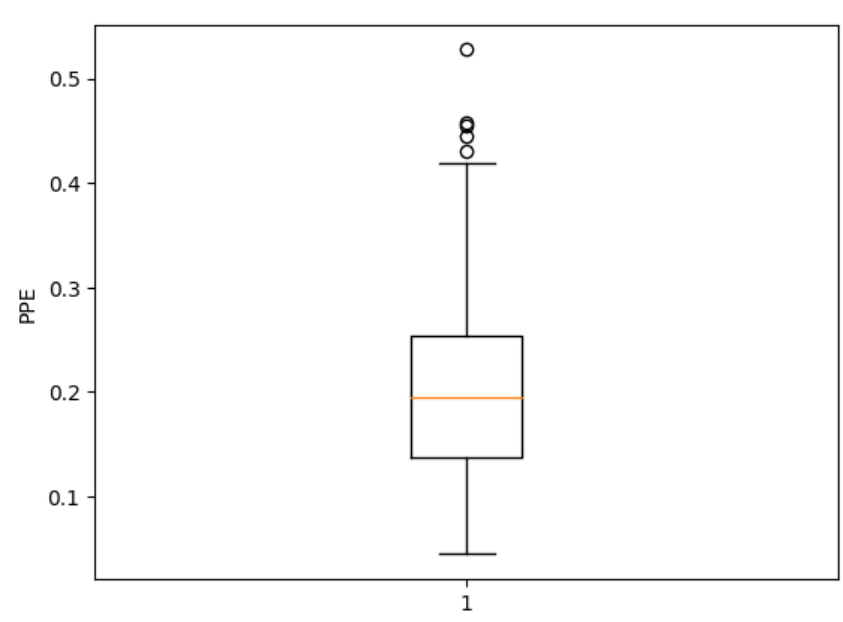
\includegraphics[height=6cm,width=8cm]{ppe.png}
    \caption{PPE boxplot}
    \label{fig:8}
 \end{figure}

 
\newpage
\section{Results Analysis}
In the experimental analysis  we have plotted the explained variance and cumulative variance.
First 5 principal components are giving 90 percent of the variance. So we have trained the model with 5 principal components. In the classification task XGBoost algorithm outperformed the decision tree.


\begin{figure}[!ht]
     \centering
     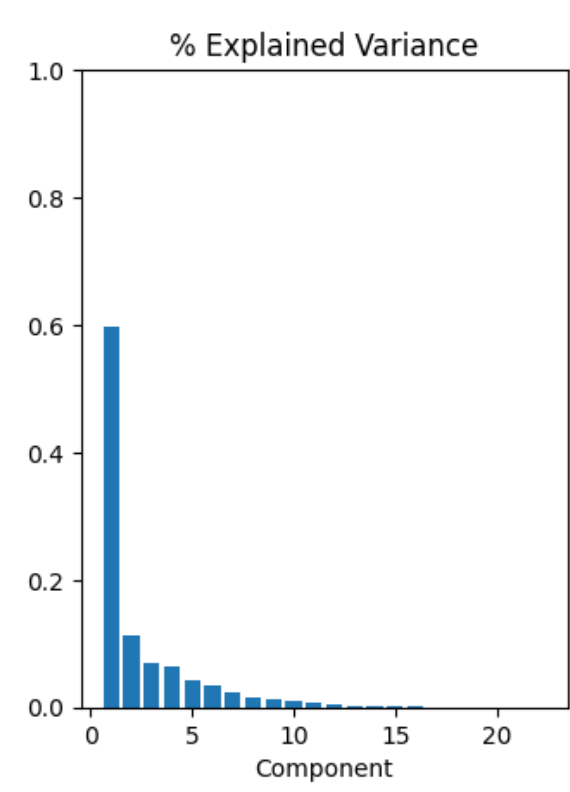
\includegraphics[height=8cm,width=8cm]{pca1.png}
     \caption{Explained variance plot}
     \label{fig:8}
 \end{figure}

 \begin{figure}[!h]
     \centering
     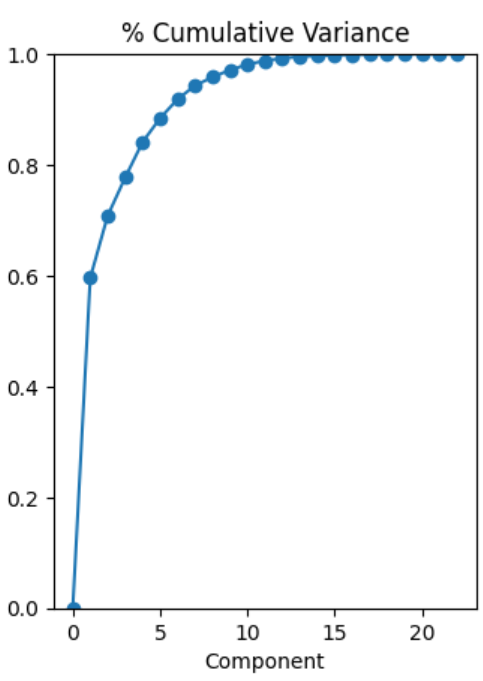
\includegraphics[height=8cm,width=8cm]{cumlative.png}
     \caption{Cumulative variance}
     \label{fig:8}
 \end{figure}


\begin{figure}[!h]
     \centering
     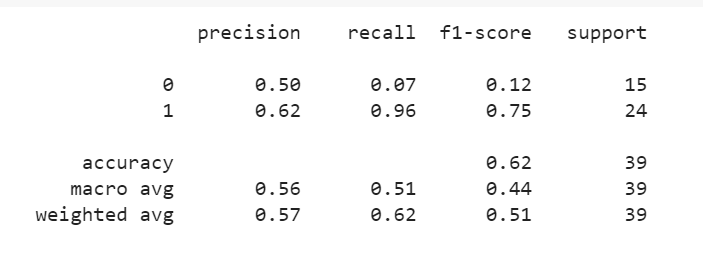
\includegraphics[height=8cm,width=8cm]{gb_classification.png}
     \caption{Gradient Boosting classification report}
     \label{fig:8}
 \end{figure}
 
\\

\begin{figure}[!h]
     \centering
     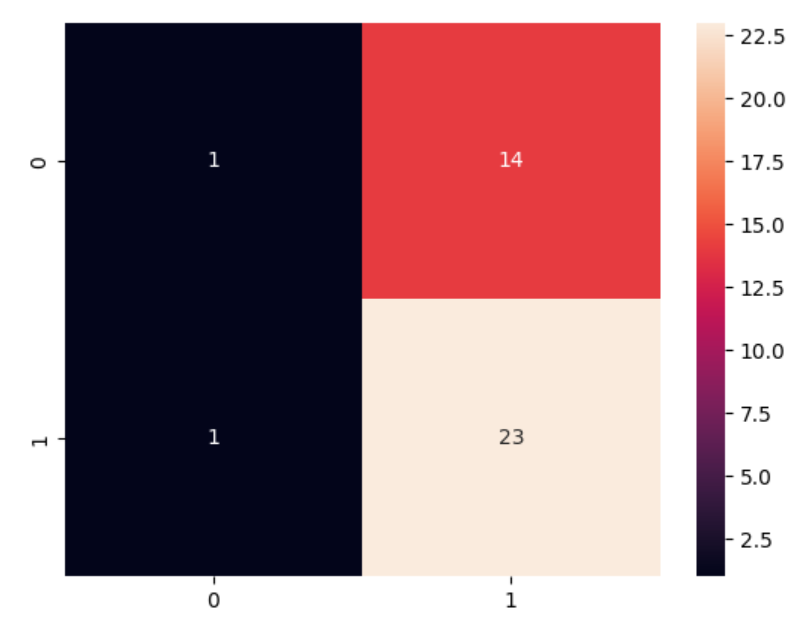
\includegraphics[height=6cm,width=8cm]{gb_conf.png}
     \caption{Gradient Boosting confusion matrix}
     \label{fig:8}
 \end{figure}
 
 
 
 
 

\section{Results summary}
Conducting the experimental analysis we can conclude that Boosting classifiers performed the best when compared to the other algorithms.So we have selected the best algorithms to implement in the web application those are Rando Forest and Gradient Boosting classifier. For better analysis of the algorithms performance we have constructed the confusion matrix for Gradient Boosting and Random Forest algorithm.
Confusion matrix gives the understanding of classification state incorrect and correct. In summary it shows where the model got confused and produced the wrong results. In the medical industry not only the accuracy for better implementation in real time we need to understand the incorrect classification as well.
Here, in the below fugures we can see the confusion matrix of Random Forest and Gradient Boosting.

In Random Forest the mis classification rate is high for moderately demented categroy and PD category compared to converted category

In Gradient Boosting  the mis classification rate is same for moderately demented categroy and PD category compared to converted category


\newpage{}
\bibliographystyle{plain}
\bibliography{references.bib}

\end{document}
